\par Tango Scrum como el resto de metodologías ágiles nacen de la necesidad de una metodología flexible y adaptable a los constantes cambios de los mercados tecnológicos \cite{bartoszScrumVideoGames2023}. Es una respuesta a las metodologías tradicionales, como Waterfall, las cuales priorizan seguir un plan definido \cite{cynthiachizobaekechiEnhancingAgileProduct2024}. En este sentido, Scrum representa un cambio de paradigma, que se enfoca en un sistema flexible, iterativo y colaborativo sobre el acercamiento basado en planes estrictos y documentación.
\par Scrum se basa en la idea de dividir el desarrollo de un software en pequeñas iteraciones llamadas sprints, generalmente durando un máximo de 4 semanas. El objetivo es que cada sprint produzca incrementalmente un producto usable, el cual puede ser presentado a un usuario final \cite{bartoszScrumVideoGames2023}.
\par Hoy en día, las empresas trabajan para crear productos digitales que satisfagan las necesidades de sus clientes, no sólo en videojuegos, si no que en la industria del software en general. Esto presenta un mayor desafío para una empresa pequeña, que aún debe competir en un mercado global a pesar de tener menos recursos \cite{putrianasariProblemsAdoptionAgileScrum2024}.Es por esto que muchas empresas implementan Scrum, una metodología que acepta el cambio constante y prepara a la institución para un ambiente dinámico y un futuro incierto \cite{putrianasariProblemsAdoptionAgileScrum2024}.
\par Scrum se basa en una serie de principios, donde los principales son:
\begin{itemize}
  \item Equipos autogestionados: a diferencia de otras metodologías, que siguen modelos jerárquicos, los equipos de Scrum tienen autoridad sobre su trabajo \cite{cynthiachizobaekechiEnhancingAgileProduct2024}. El objetivo es generar colaboración y responsabilidad por parte de los integrantes.
  \item Desarrollo iterativo: los proyectos que aplican Scrum se construyen en base a múltiples iteraciones del producto, mejorando la funcionalidad y calidad en cada una de ellas. El objetivo es motivar la adaptación continua de feedback, y la posibilidad de responder a cambios de manera rápida y efectiva \cite{cynthiachizobaekechiEnhancingAgileProduct2024}.
  \item Enfoque en el usuario final: con Scrum se busca involucrar al usuario en cada iteración del producto, de forma que esté alineado con las demandas del mercado \cite{cynthiachizobaekechiEnhancingAgileProduct2024}.
\end{itemize}
%
%
\subsection{Equipos}
\par En Scrum, el equipo consiste de 3 partes, el \emph{Scrum Master}, el \emph{Product Owner} y los \emph{Developers}. Todas las partes trabajan para cumplir un objetivo en común, llamado \emph{Product Goal} \cite{schwaberScrumGuide2020}. Además, se encuentra el rol de los \emph{Stakeholders}, que alinean al equipo a las demandas del mercado \cite{schwaberScrumGuide2020}.
\par Los equipos de Scrum son autogestionados, es decir que los miembros deciden en conjunto el itinerario de tareas, y las responsabilidades de cada uno. Se recomienda que el tamaño del equipo no supere las 10 personas, ya que de otra forma se complica la comunicación y la autonomía.
\subsubsection{Developers}
\par El equipo de \emph{Developers} se encarga de trabajar en cualquier aspecto de un \emph{Increment} en cada \emph{Sprint}. Sus tareas consisten en crear un plan para el \emph{Sprint}, llamado \emph{Sprint Backlog}, y llevarlo a cabo, considerando lo indicado por el \emph{Definition of Done}.
%
\subsubsection{Product Owner}
\par El \emph{Product Owner} se encarga de manejar el \emph{Product Backlog}. Este rol implica la creación, priorización y comunicación constante deeste mismo, asegurando que refleje las necesidades del cliente y los objetivos estratégicos del negocio.
\par Este rol suele ser ocupado por una sola persona, y puede representar las necesidades de varios \emph{Stakeholders}.
%
\subsubsection{Scrum Master}
La tarea del \emph{Scrum Master} es establecer las prácticas de Scrum y asegurarse de que el equipo las cumpla. Su objetivo es facilitar la implementación de la metodología. Cabe destacar que no es un rol de liderazgo, si no que trabaja como facilitador, ayudando al equipo a resolver impedimentos y mejorar su rendimiento.
\subsubsection{Stakeholders}
\par Se considera un \emph{stakeholder} a cualquier entidad que esté interesada en el éxito del producto. Ejemplos de \emph{stakeholders} son:
\begin{itemize}
  \item Clientes y usuarios finales
  \item Inversores
  \item Proveedores y vendedores
\end{itemize}
%
%
\subsection{Eventos}
\par Scrum busca promover una cultura de mejora continua, donde el equipo pueda aprender de sus experiencias y mejorar a futuro \cite{excelgchukwurahELEVATINGTEAMPERFORMANCE2024}. Es por esto que se establecen varios eventos que ayudan al equipo a mantenerse enfocado y en constante evolución.
%
\subsubsection{Sprints}
\label{sec:sprint}
\par Las tareas del equipo se dividen en pequeñas iteraciones llamadas \emph{sprints}, generalmente durando un máximo de 4 semanas. El objetivo es que cada sprint produzca incrementalmente un producto usable, el cual puede ser presentado a un \emph{stakeholder} \cite{bartoszScrumVideoGames2023}.
\par Durante un \emph{Sprint} no pueden realizarse cambios a las tareas. El scope del próximo \emph{Sprint} puede ser renegociado en base a lo aprendido en el actual. Sólo un \emph{Product Owner} puede cancelar un \emph{Sprint}, en caso de que sea necesario.
%
\subsubsection{Sprint Planning}
\par Evento que inicia el \emph{Sprint}, donde se decide el trabajo que se realizará en este mismo. Este plan es creado por el \emph{Scrum Team}. El \emph{Product Owner} debe asegurarse que los miembros del equipo estén preparados para discutir los ítems más importantes del \emph{Product Backlog}. Los objetivos del \emph{Sprint planning} son:
\begin{itemize}
  \item Definir el \emph{Sprint Goal}.
  \item Seleccionar los ítems del \emph{Product Backlog} que se trabajarán durante el \emph{Sprint}.
  \item Desglosar las tareas seleccionadas del \emph{Product Backlog} en ítems pequeños, que no tomen más de un día de trabajo. Esto es llevado a cabo exclusivamente por los \emph{Developers}.
\end{itemize}
%
\subsubsection{Daily Scrum}
Reuniones diarias de 15 minutos donde los \emph{Developers} inspeccionan el trabajo del \emph{Sprint} y lo ajustan en caso de ser necesario. Cada desarrollador comparte su progreso y las tareas que realizará ese día \cite{bartoszScrumVideoGames2023,schwaberScrumGuide2020}.
%
\subsubsection{Sprint Review}
En este evento, el \emph{Scrum Team} presenta los resultados del \emph{Sprint} a los \emph{stakeholders}. Luego, se revisa qué se completó durante el \emph{Sprint}, y se evalúa si la dirección en la que se está trabajando cumple el \emph{Product Goal}.
%
\subsubsection{Sprint Retrospective}
Evento final que concluye el \emph{Sprint}. El \emph{Scrum Team} evalúa el progreso del mismo, investigando procesos, herramientas y el trabajo realizado. También se discute los aspectos positivos y negativos del \emph{Sprint}, y se encuentran formas de mejorar sobre las dificultades encontradas.
%
%
\subsection{Artefactos}
%
\subsubsection{Product Backlog}
\par Lista ordenada de tareas necesarias para llevar a cabo un producto. Representa el trabajo llevado a cabo por el \emph{Scrum Team}. Esta lista es constantemente refinada por el \emph{Product Owner} \cite{cynthiachizobaekechiEnhancingAgileProduct2024}, añadiendo detalles a las tareas, separándolas en ítems más precisos o cambiando el orden y prioridad.
\par El objetivo de este artefacto es asegurarse que el equipo se enfoque en las tareas más importantes, que generen la mayor cantidad de valor para el usuario final \cite{cynthiachizobaekechiEnhancingAgileProduct2024}.
%
\subsubsection{Product Goal}
\par Primero, se define a un producto como un objeto que produce valor para un usuario final \cite{schwaberScrumGuide2020}. Se considera entonces un \emph{Product Goal} al objetivo final que el \emph{Scrum Team} planea llevar a cabo. Es el objetivo a largo plazo del equipo.
%
\subsubsection{Sprint Backlog}
\par Set de ítems del \emph{Product Backlog} que se espera completar durante el \emph{Sprint}. Es creado y mantenido por los \emph{Developers}.
%
\subsubsection{Sprint Goal}
Objetivo del \emph{Sprint actual}, creado en el \emph{Sprint Planning}. Las tareas del \emph{Sprint Backlog} se deciden en torno a esta meta.
%
\subsubsection{Increment}
\par Artefacto que representa un paso hacia el \emph{Product Goal}. Son aditivos, es decir que se construyen en base a \emph{Increments} anteriores. Se presentan durante el \emph{Sprint Review} como evidencia empírica del trabajo realizado. Los incrementos se crean cuando un ítem del \emph{Product Backlog} cumple el \emph{Definition of Done}.
%
\subsubsection{Definition of Done}
Este artefacto describe los estándares de calidad a los que debe llegar el trabajo actual para ser considerado un \emph{Increment}.
%
\subsubsection{Story Point}
\par Los \emph{Story Points} son una unidad de medida que se utiliza para estimar el esfuerzo necesario para completar una tarea. En Scrum, se utilizan para medir la complejidad y el tamaño relativo de las tareas en el \emph{Product Backlog}. Los equipos asignan puntos a cada tarea en función de su dificultad, lo que les permite priorizar y planificar mejor el trabajo \cite{montegalianoImplantarScrumCon2016,canosaferreiroSCRUMTeoriaImplementacion2024}. 
%
\subsubsection{Burndown Chart}
\label{sec:burndown_chart}
\par Gráfico que muestra el progreso del equipo durante un periodo de tiempo. En Scrum, se utiliza para visualizar el trabajo restante en un \emph{Sprint} (llamado \textit{Sprint burndown}) o en un proyecto completo (llamado \textit{release burndown}). El eje X representa el tiempo, mientras que el eje Y muestra la cantidad de trabajo restante, generalmente medido en \emph{story points} o en horas de trabajo \cite{montegalianoImplantarScrumCon2016,canosaferreiroSCRUMTeoriaImplementacion2024}. 
%
\begin{figure}[h]
    \centering
    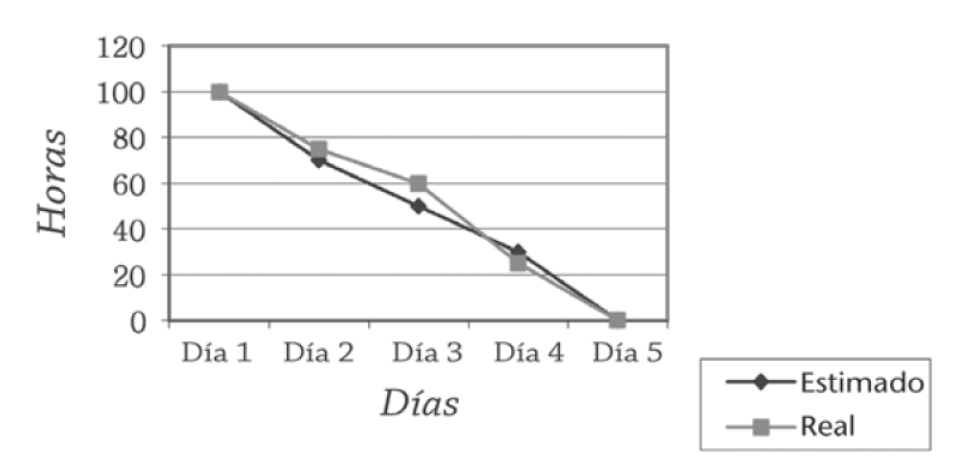
\includegraphics[width=.49\textwidth]{burndown_sprint.png}
    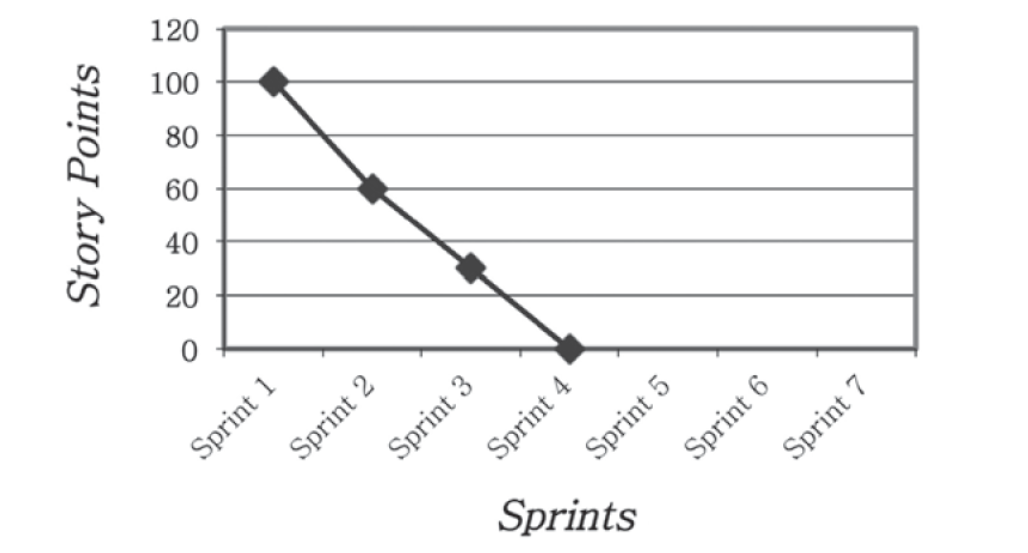
\includegraphics[width=.49\textwidth]{burndown_release.png}
    \caption{Ejemplo de un \textit{sprint burndown} (izquierda) y un \textit{release burndown} (derecha). Extraída de \cite{montegalianoImplantarScrumCon2016}.}
    \label{fig:x sprint burndown ejemplo}
\end{figure}
%
%
\subsection{Dificultades de Scrum}
\subsubsection{En el software tradicional}
\par Si bien varias organizaciones han sido impactadas positivamente por la implementación de Scrum, otras se han encontrado con dificultades. En 2020 se realizó una investigación que estima que la metodología falló en el 84\% de compañías pequeñas-medianas que lo implementaron \cite{putrianasariProblemsAdoptionAgileScrum2024}.
\par Putrianasari et al. \cite{putrianasariProblemsAdoptionAgileScrum2024} menciona 4 áreas en las que las compañías fallan a la hora de implementar Scrum.
\bigbreak
{\setlength{\parindent}{0cm}Manejo de personal}
\bigbreak
\par Una de las principales problemáticas es la falta de colaboración y comunicación en los equipos. Los desarrolladores tienden a enfocarse en sus objetivos individuales y pierden de vista los objetivos de la organización. Además, al tratarse de empresas pequeñas-medianas, los empleados rotan entre varios proyectos, cambiando constantemente de equipo. Esto va en contra de uno de los pilares de Scrum, donde el equipo debe ser autónomo, decidiendo sus tareas y evaluando su propio progreso \cite{putrianasariProblemsAdoptionAgileScrum2024}.
\bigbreak
\par Por otro lado, la resistencia al cambio por parte de los empleados puede traer problemas a la hora de implementar Scrum eficientemente. Esto viene de la falta de conocimiento de la metodología, un equipo de tamaño incorrecto, o de la falta de compromiso por parte de los trabajadores \cite{putrianasariProblemsAdoptionAgileScrum2024}.
\bigbreak
{\setlength{\parindent}{0cm}Proceso de adopción}
\bigbreak
\par Varias dificultades pueden aparecer a la hora de llevar a cabo la implementación. Una de ellas, la falta de comprensión de los conceptos y principios de Scrum. La investigación nota que algunas organizaciones ven el éxito que la metodología trae a otras empresas y se apresuran a implementarlo sin analizar cómo ayudaría en sus procesos de desarrollo.
\bigbreak
{\setlength{\parindent}{0cm}Problemas organizaciones}
\bigbreak
\par Para implementar Scrum exitosamente, las empresas deben dar una definición de éxito y alinear las prácticas de Scrum con los objetivos de la organización. Al fallar en alguno de estos procesos, la metodología no puede ser aplicada correctamente.
\bigbreak
{\setlength{\parindent}{0cm}Problemas técnicos}
\bigbreak
\par En algunos casos se nota que las empresas no utilizan herramientas y tecnología que facilitan la implementación de Scrum. Además, se observan casos donde el presupuesto prestado para establecer la metodología no cubre estas tecnologías.
%
\subsubsection{Scrum-but}
\par Si bien la guía de Scrum dictamina que se deben evitar cambios a sus estructuras \cite{schwaberScrumGuide2020}, las prácticas de esta metodología rara vez son seguidas de forma consistente \cite{HawaiiInternationalConference2020}. Es común ver implementaciones parciales de Scrum, donde sólo se aplican ciertos eventos o artefactos.
Hassani-Alaoui et al. \cite{HawaiiInternationalConference2020} identifica 3 situaciones donde el éxito de un proyecto se ve afectado por desviar de las prácticas de Scrum:
\begin{enumerate}
    \item La calidad del producto se ve afectada cuando un equipo no es autónomo. idealmente, los miembros del equipo se encargan de planear el sprint. Sin embargo, hay ocasiones donde esta responsabilidad pasa al Product Owner, Scrum Master, o alguna posición de manager similar. Esta pérdida de control se puede traducir en estimaciones incorrectas y por lo tanto una mala performance del equipo.
    \item El product owner debe ser el único responsable de manejar el product backlog. Cuando el product owner no es capaz de organizar y planear el backlog, el equipo no es capaz de trabajar en los ítems que el cliente desea priorizar.
    \item Las retrospectives son importantes para tener un paso de reflexión y mejora de los procesos de trabajo. En los casos donde esta reunión no se realizaba, o se utilizaba para expresar frustraciones en vez de buscar soluciones para ellas, se pudo observar una pérdida de eficiencia y efectividad.
\end{enumerate}
\par Por otro lado, Ramirez Lathi et.al \cite{lahtiScrumButIndicatorProcess2022} encuentra una relación entre anti-patrones a la hora de desarrollar un software y la aplicación de Scrum-but. Su investigación muestra cómo una empresa que evita algunos de los artefactos importantes, como Sprints o Testing, genera código que es propenso a errores y deuda técnica.